\documentclass[12pt]{article}
\usepackage{graphicx}
\begin{document}
\section{Introduction}
A network is an abstract construct, capturing the relation (links) between entities (nodes).
This simplified way of displaying relations has proven useful in many areas of science, humanities and everyday life. 
Networks are all around us, from the intricate interactions of thousands of organisms in an ecosystem, to virtual social networks on the web, networks are an inseparable element of our everyday lives. 

\section{Methodology}
Our goal with this project was to bring networks to life as physical objects, a testimony to their physical reality in spite of being an abstract mathematical construct. 
In visualizing networks nodes are generally represented as point-like objects and links as lines.  
We aimed to add a “physicality” to the nodes and links to create a manifestation of a network in form of a three dimensional object. 
This presented a number of challenges due to the fact that links and nodes have to occupy space, resulting in multiple crossings between nodes and links. 
To avoid such conflicts we developed a novel layout algorithm which uses physical forces to push conflicting nodes and links apart from each other.
Additionally, we wanted the algorithm to find the most economical layout possible, in the sense that links are as short as possible while avoiding overlap. 
To achieve this, we modelled links as elastic tubes, which repel each other to avoid overlaps, but also bend and curve to find the shortest paths connecting their end nodes, similar to self-avoiding polymers \cite{des1974lagrangian}.
We also wanted nodes to not only avoid crossing each other, but also that each node has sufficient empty space around it. 
We, therefore, introduce short-range repulsion forces to make sure nodes do not come closer than a minimum distance, which we adjust based on the number of links connected to the node. 
We encode all of these forces in a ``potential energy’’ function, which plays the role of a cost function. 
To achieve a desirable layout, we dynamically simulate the physical forces by performing gradient descent on the potential energy. 
To avoid, bad local minima, we run simulated annealing \cite{kirkpatrick1987optimization}, which adds thermal fluctuations that allow the system to escape undesirable states. 
\begin{figure}
    \centering
    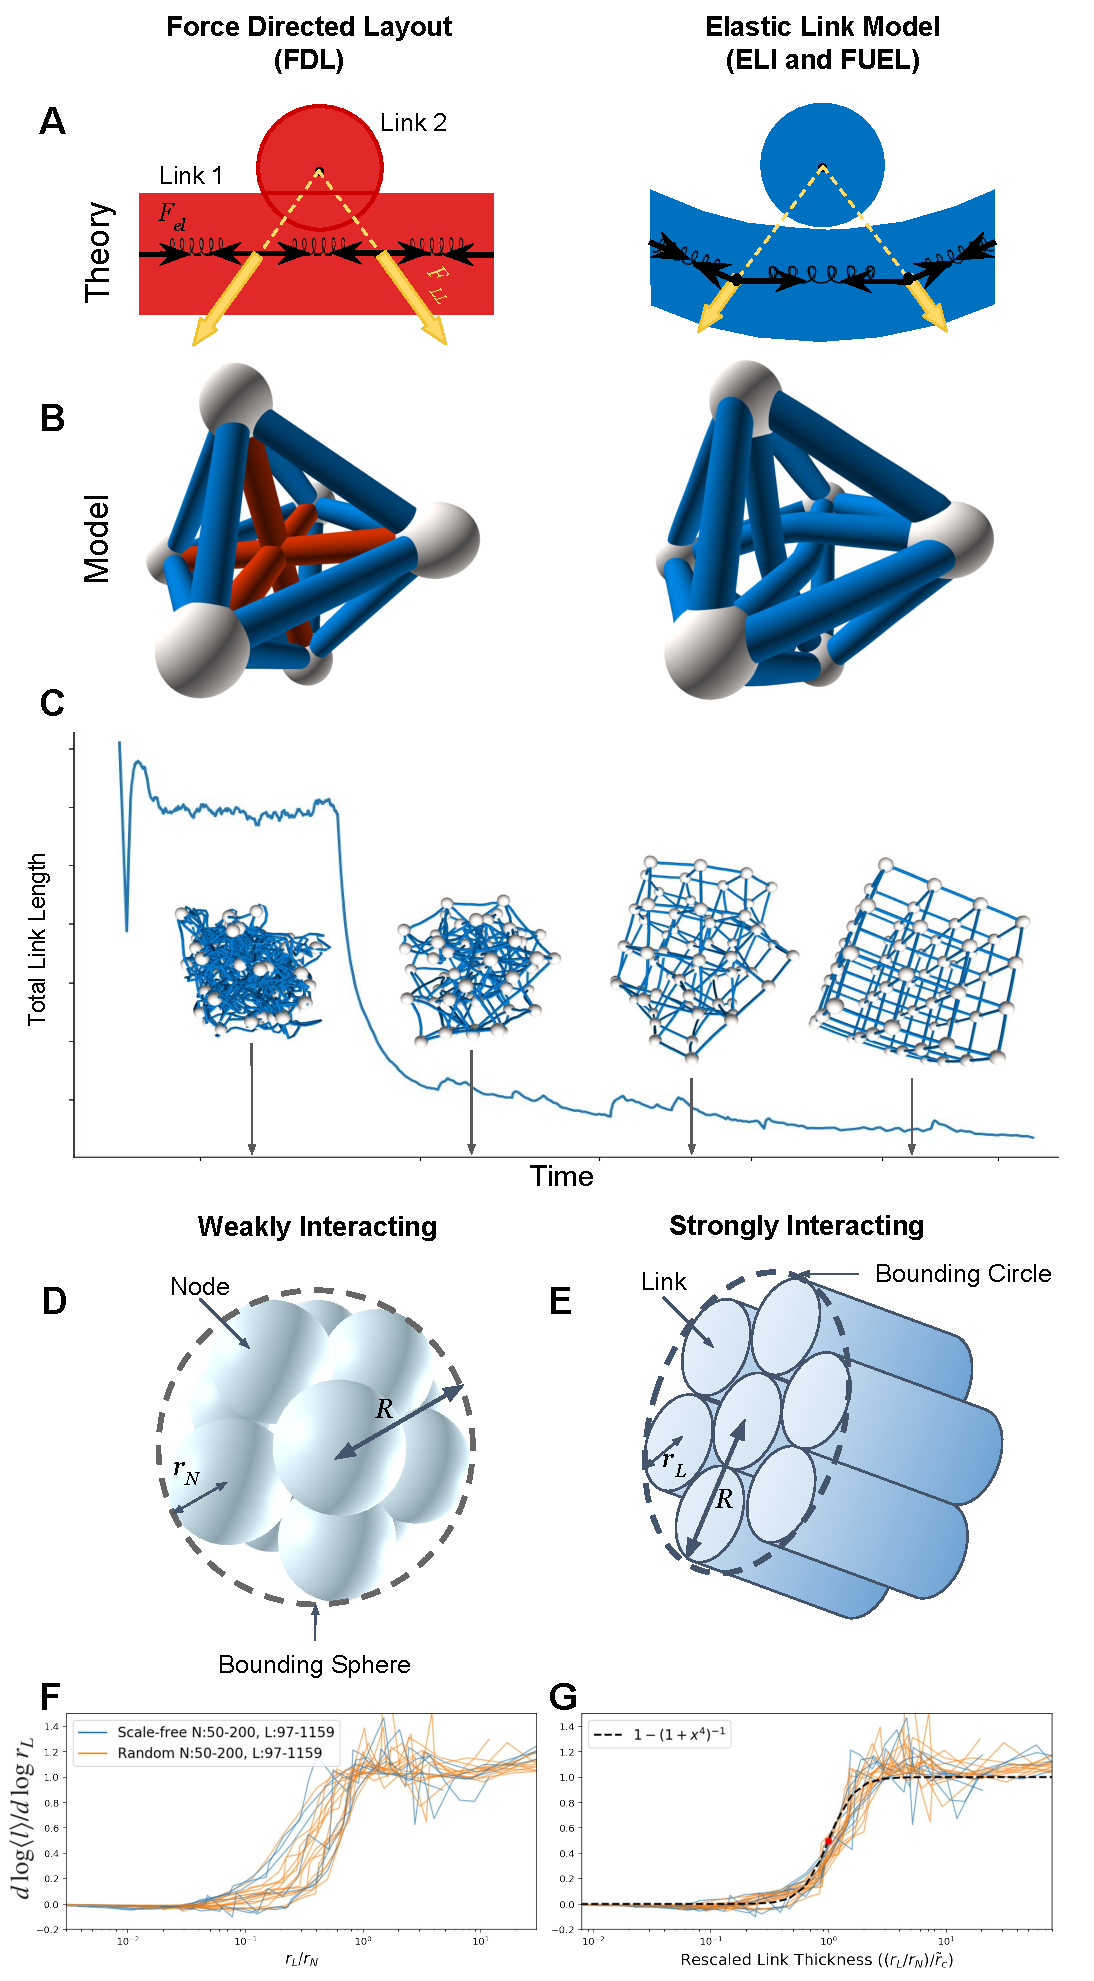
\includegraphics[width=.78\columnwidth, trim=0 12.5cm 0 0cm,clip]{fig-09-19/3d-crs-lat-trans-041018.pdf}
    \caption{
    \scriptsize
    {\bf(A) Modeling Framework:} We model each link as a stretched, flexible rubber band, 
    corresponding to many short springs connected to each other, pulled apart by
    elastic forces $F_{el}$. 
    The links exert a repulsive force $F_{LL}$  on each other that falls sharply at radii larger than $r_L$. 
    While in FDL the links cross each other (left figure), in ELI and FUEL such crossings are prohibited (right figure). 
    {\bf(B)} A small network with $N=6$ nodes laid out with FDL (left), resulting in multiple link crossings, shown as red links.   
    The right plot shows how the network laid out by ELI that resolves the crossings.
    {\bf (C)} Finding the final layout of a lattice with $r_L\ll r_N$, also showing the evolution of the total link length over time during the simulation. 
    We started from a random layout and used simulated annealing to find the final layout.
    The thermal noise helps links pass through each other and resolve crossings.}
    \label{fig:my_label}
\end{figure}

\bibliographystyle{plain}
\bibliography{mybib}


\end{document}